\documentclass[conference]{IEEEtran}
\IEEEoverridecommandlockouts
\usepackage{cite}
\usepackage{amsmath,amssymb,amsfonts}
\usepackage{algorithmic}
\usepackage{graphicx}
\usepackage{textcomp}
\usepackage{xcolor}
\usepackage{array}
\usepackage{subfig}
\usepackage{stfloats}
\usepackage{url}
\usepackage{verbatim}
\usepackage{booktabs}
\usepackage{multirow}
\usepackage{xspace}
\usepackage{colortbl}
\usepackage{siunitx}
\usepackage{pgfplots}
\pgfplotsset{compat=1.18}
\usepackage{tikz}
\usetikzlibrary{shapes,arrows,positioning,fit,arrows.meta,calc,backgrounds}
\usepackage[hidelinks]{hyperref}
\usepackage{orcidlink}
\def\BibTeX{{\rm B\kern-.05em{\sc i\kern-.025em b}\kern-.08em
T\kern-.1667em\lower.7ex\hbox{E}\kern-.125emX}}
\begin{document}

\title{A Training and Evaluation Methodology for Robust DGA Detection}

\author{\IEEEauthorblockN{Reynier Leyva La O\orcidlink{0000-0003-3975-1437}}
\IEEEauthorblockA{\textit{GridTICs, Facultad Regional Mendoza} \\
\textit{Universidad Tecnológica Nacional}\\
Mendoza, Argentina \\
rleyvalao@mendoza-conicet.gob.ar}
\and
\IEEEauthorblockN{Carlos A. Catania\orcidlink{0000-0002-1749-310X}}
\IEEEauthorblockA{\textit{LABSIN, Facultad de Ingeniería} \\
\textit{Universidad Nacional de Cuyo}\\
Mendoza, Argentina \\
\textit{CONICET}\\
harpo@ingenieria.uncuyo.edu.ar}
}

\maketitle

\begin{abstract}
Most DGA detection papers evaluate models on small, inconsistent benchmarks that say little about how a detector will behave on new malware families. Fair comparison across papers is difficult, and a key question goes unanswered: does a model learn general DGA behavior, or does it memorize the families it was trained on? We propose an evaluation methodology organized around four scenarios: seen families, word list families within the seen set, unseen families, and unseen word list families as the hardest case. Inference time and behavior under class imbalance are reported as deployment considerations. We apply this methodology to seven models, from logistic regression to fine-tuned transformers, trained on 54 DGA families and evaluated on all 79 in the study, with 25 kept completely unseen to measure generalization. The protocol uses 30 independent runs per family. Rankings change substantially across scenarios. A model that ranks first on seen families can drop to sixth on unseen ones. Word list families remain hard even for language models, and under a realistic 1:100 traffic ratio the best result across all models is F1~=~0.182. A single test set is not enough to characterize a detector.
\end{abstract}

\begin{IEEEkeywords}
domain generation algorithms, DGA detection, evaluation methodology, generalization, transformers, DNS security, malware detection
\end{IEEEkeywords}

\section{Introduction}
\label{sec:introduction}

Malware operators use domain generation algorithms (DGAs) to keep their infrastructure alive when defenders try to take it down. Rather than connecting to a fixed server, infected machines compute a list of candidate domain names from a secret seed and try each one until they find an active command and control (C\&C) host. Defenders can block individual domains or redirect traffic through sinkholes, but they cannot block every name in a list that may contain tens of thousands of entries per day.

This technique has been in use for over fifteen years. In early 2024, ESET documented the takedown of Grandoreiro and reported 105 DGA configurations, 79 active C\&C servers, and sinkholing data that revealed around 563 victims per day across three countries~\cite{eset2024grandoreiro}. Only weeks later, IBM X-Force reported that Grandoreiro had returned with a new DGA using 14 seeds that generates 14 candidate domains per day~\cite{ibm2024grandoreiro}. In late 2024, Zscaler found that ZLoader 2.9.4.0 combined DGA with Domain Name System (DNS) tunneling, producing 32 domains per day while hiding traffic inside encrypted DNS communication~\cite{zscalerzloader2024}. Forescout reported that 75\% of malicious command and control domains in its study were generated algorithmically~\cite{forescout2025}.

Classifying a domain as DGA-generated or legitimate from its name alone is the most practical approach at the DNS layer, where every query passes before reaching any application. Work on this problem goes back to at least 2010~\cite{plohmann_dga, yadav2010detecting}, and the literature now covers a wide range of methods: logistic regression on hand-crafted features~\cite{Soleymani_LGic}, character-level convolutional networks~\cite{catania2019analysis}, recurrent models with attention~\cite{tuan2022detecting}, transformer-based models fine-tuned on domain data~\cite{mahdaouy2024domurls_bert, Dom-BERT}, and more recently large language models adapted for domain classification~\cite{la2024llms, alqahtani2025llmreview}.

With all this work, one would expect a clear picture of which detectors work and under what conditions. That picture does not exist. Cebere et al.~\cite{cebere2024down} surveyed 38 DGA detection papers and found that most rest on fragile experimental foundations: different papers use different family subsets, different non-DGA datasets, and different metrics. More critically, 64\% of papers do not test their models on families absent from training, 87\% report no inference time, and most papers skip word list families, which are the hardest to detect. The result is that a published number cannot tell you whether a model learned general DGA behavior or memorized the families it was trained on, let alone whether it would hold up against the hardest cases in a real deployment.

Cebere et al. identified these gaps but did not close them. Their contribution was a diagnosis. Ours is the evidence: we show that these missing evaluations are not just oversights, they change the conclusions. We apply a concrete evaluation methodology to seven models across 79 DGA families, and the results are hard to ignore. A model that ranks first on known families can rank sixth on unseen ones. The simplest model in the study generalizes better than the most expressive one. These reversals are invisible under the single-benchmark evaluation that most papers use.

All seven models are trained on the same 54 families and evaluated under a common protocol of 30 independent runs per family. Evaluation covers two splits: the 54 training families and 25 completely unseen families for generalization. Within each split, we analyze all families together and word list families in isolation, since these are systematically harder and most papers skip them entirely, resulting in four evaluation scenarios in total. Inference time and performance under class imbalance are reported separately, as deployment considerations relevant regardless of which families a model has seen.             
          
Our main contributions are:

\begin{enumerate}
\item A curated dataset of \textbf{79 DGA families}: 54 for training with approximately one million labeled domains balanced against legitimate traffic from the Tranco list~\cite{tranco}, and 25 kept completely unseen for generalization testing, including word list and hard cases.
\item An \textbf{evaluation methodology organized around four scenarios} that follow from testing each model on two splits (seen and unseen families) and analyzing word list families separately within each split, complemented by systematic reporting of inference time and class imbalance behavior.
\item A \textbf{systematic comparison of seven models} from logistic regression to transformer encoders, trained and evaluated under the same fixed protocol across all 79 malware families.
\end{enumerate}

\section{Related Work}
\label{sec:related}

DGA detection started with hand-crafted statistical features and classical classifiers~\cite{yadav2010detecting, schuppen2018fanci, vranken2022tfidf}, then moved to character-level deep learning~\cite{catania2019analysis, woodbridge2016predicting, tuan2022detecting, yu2018character}, and more recently to transformer-based models~\cite{mahdaouy2024domurls_bert, la2024llms, alqahtani2025llmreview}. Each generation reported better numbers, but on different benchmarks and family sets, so direct comparison across papers has always been difficult. Word list families add another layer of difficulty: their domains are built from real dictionary words and look close to legitimate traffic, which makes character-level models unreliable on them~\cite{highnam2021realtime, satoh2021word}.

The deeper issue is that inconsistent evaluation hides real weaknesses. Classifier rankings change with dataset composition and evaluation settings~\cite{sivaguru2019evaluation, zago2020scalable}, and most studies only test models on families seen during training, which gives an optimistic picture of real-world behavior~\cite{lu2025transformer, duc2025federated}. Cebere et al.~\cite{cebere2024down} documented this most carefully, showing that generalization to unseen families, word list performance, and inference time are rarely measured together. Public datasets~\cite{zago2020umudga, tuan2023utldga22} and shared frameworks~\cite{pelayo2025rampage} have made experiments more reproducible, but reproducibility alone does not fix a benchmark that never tests the hard cases. This paper directly addresses those gaps.

\section{Evaluation Methodology}
\label{sec:design}

\subsection{Dataset}

We use three data partitions. The training set contains 54 DGA families: 46 non-word list (NW) and 8 word list (WL). Each family contributes 10,000 DGA     
  domains, giving 540,000 DGA samples in total. An equal number of legitimate domains are drawn from the Tranco top sites list~\cite{tranco}, for a combined  
  total of 1,080,000 labeled samples. We use a 1:1 ratio to prevent models from exploiting class imbalance during training; the effect of more realistic      
  ratios is measured in Section~\ref{sec:imbalance}. DGA domains come from DGArchive~\cite{plohmann2015dgaarchive}, 360 Netlab~\cite{360netlab},              
  UMUDga~\cite{zago2020umudga}, and UTL\_DGA22~\cite{tuan2023utldga22}.                                                                                        
                                                                                                                                                              
  The second partition is the seen test set. It covers the same 54 families used for training, but uses a separate sample: 30 independent runs per family,    
  each drawing 50 DGA domains and 50 legitimate domains. The legitimate domains are the same fixed pool of 1,500 samples paired with each family.             
   
  The third partition is the unseen test set. It contains 25 families never seen during training: 21 NW and 4 WL. The evaluation protocol is the same, 30 runs
   of 50 DGA and 50 legitimate per family, but the legitimate domains are a different pool from the one used in the seen test set. No samples from these 25
  families are used for training or model selection. Their only purpose is to measure how well each model generalizes to families it has never encountered.   
                                         

Word list families deserve a separate note. They generate domains by concatenating real dictionary words, producing strings that look like natural language~\cite{plohmann_dga, leyva2026expert}. A domain like \texttt{lookbitterboyfriend.tel} carries no statistical anomaly in character frequencies or n-gram distributions, so purely character-level models cannot detect it reliably. Including WL families in both splits lets us measure this difficulty under both standard and out-of-distribution conditions.

For character-level models, domain strings are lowercased and truncated or padded to a fixed length of 64--75 characters using a vocabulary of printable ASCII characters. For transformer models, we use the tokenizer provided with each pretrained checkpoint without modification.                               
  


Table~\ref{tab:families} lists all 79 families grouped by split and type.

\begin{table}[!t]
\caption{DGA families used in the study. The 54 training families are split into 8 WL and 46 NW. The 25 generalization families include 4 WL and 21 NW.}
\label{tab:families}
\centering
\renewcommand{\arraystretch}{1.15}
\resizebox{\linewidth}{!}{%
\begin{tabular}{p{1.8cm} p{6.3cm}}
\toprule
\textbf{Split / Type} & \textbf{Families} \\
\midrule
Train WL (8) &
charbot, deception, gozi, manuelita, matsnu, nymaim, rovnix, suppobox \\
\addlinespace
Train NW (46) &
alureon, bamital, banjori, bedep, chinad, conficker, corebot,
cryptolocker, dircrypt, dnschanger, dyre, emotet, fobber,
gameover, kraken, locky, monerominer, murofet, murofetweekly,
mydoom, necurs, oderoor, padcrypt, pitou, proslikefan, pushdo,
pykspa, qadars, qakbot, qsnatch, ramdo, ramnit, ranbyus, shiotob,
simda, sisron, sphinx, symmi, tempedreve, tinba, tinynuke,
vawtrak, vidro, virut, zeus-newgoz, zloader \\
\addlinespace
New WL (4) &
bigviktor, gozi\_rfc4343, pizd, ngioweb$^*$ \\
\addlinespace
New NW (21) &
bazarbackdoor, bazarbackdoor\_v2, bazarbackdoor\_v3, bumblebee,
ccleaner, dmsniff, enviserv, fosniw, goz, infy, monerodownloader,
newgoz, pandabanker, reconyc, sharkbot, szribi, torpig, tufik,
verblecon, wd, xshellghost \\
\bottomrule
\multicolumn{2}{p{\linewidth}}{\footnotesize
$^*$ngioweb uses real prefixes (mini-, sub-) with invented word bodies.
It does not use dictionary words directly but is treated as WL in the
generalization set.}
\end{tabular}}
\end{table}

\subsection{Compared Models}

Table~\ref{tab:models} summarizes the seven models, which span from a simple logistic regression baseline to large transformer encoders, covering several orders of magnitude in parameter count and inference cost.

\begin{table}[!t]
\caption{Models included in the study. All character-level models use a maximum domain length of 64--75 characters. Inference times are measured per domain on a single CPU thread (Google Colab)~\cite{google_colab}.}
\label{tab:models}
\centering
\renewcommand{\arraystretch}{1.1}
\resizebox{\linewidth}{!}{%
\begin{tabular}{lllr}
\toprule
\textbf{Model} & \textbf{Architecture} & \textbf{Framework} & \textbf{Params} \\
\midrule
CNN & Conv1D (64 filters) + MaxPool + FC~\cite{catania2019analysis} & PyTorch & $\sim$50\,K \\
BiLSTM & BiLSTM + self-attention~\cite{namgung2022efficient} & PyTorch & $\sim$700\,K \\
Bilbo & CNN + LSTM~\cite{highnam2021real} & PyTorch & $\sim$1.5\,M \\
Logit & TF-IDF (char 3--5-grams) + LR~\cite{Vranken_mdpi} & sklearn & $\sim$8\,M \\
LA\_Bin07 & BiLSTM + SeqWeightedAttention~\cite{la2024llms} & Keras & $\sim$8\,M \\
DomURLs-BERT & BERT-base + LoRA ($r$=8)~\cite{mahdaouy2024domurls_bert} & HF & 110\,M \\
ModernBERT & ModernBERT-base, fine tuned~\cite{modernbert_hf_2024} & HF & 149\,M \\
\bottomrule
\end{tabular}}
\end{table}

\subsection{Training}

Neural character-level models (CNN, BiLSTM, Bilbo, LA\_Bin07) are trained from scratch using Adam~\cite{kingma2014adam} with learning rate $10^{-3}$, batch size 256, and early stopping with patience 5 on a held-out 10\% of the training set. The logistic regression baseline uses TF-IDF character 3--5-grams with a SAGA solver. Both transformer models are fine-tuned using LoRA ($r=8$, $\alpha=16$) with AdamW, learning rate $2 \times 10^{-4}$, and batch size 32 for 5 epochs. The generalization set is never used during training or for checkpoint selection.

All experiments use PyTorch 2.1, Keras 3.0, scikit-learn 1.4, and Hugging Face Transformers 4.40. Code, trained models, and dataset splits are available at~\cite{reynier_dga_multifamily_benchmark} upon publication.

\subsection{Evaluation Protocol}

Figure~\ref{fig:methodology} shows the full structure of the evaluation. Every model is tested under the same conditions, so results are directly comparable regardless of architecture.

\begin{figure*}[!t]
\centering
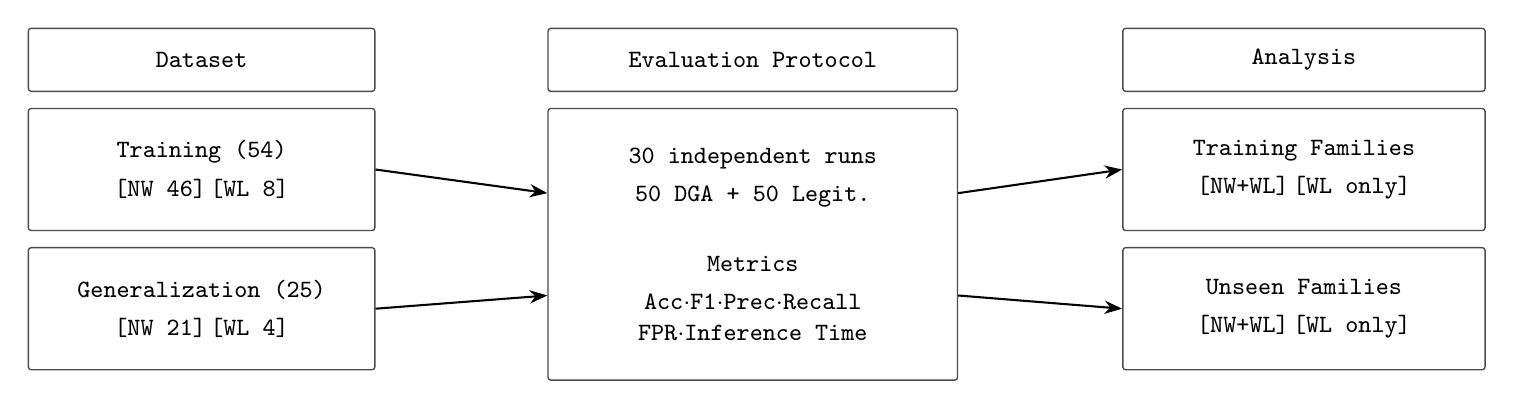
\begin{tikzpicture}[
    font=\small\ttfamily,
    >=Stealth,
    head/.style={
        draw=black!70,
        rounded corners=1pt,
        minimum width=#1,
        minimum height=0.8cm,
        align=center,
        line width=0.5pt
    },
    card/.style={
        draw=black!70,
        rounded corners=1pt,
        minimum width=#1,
        minimum height=1.55cm,
        align=center,
        inner sep=6pt,
        line width=0.5pt
    },
    proto/.style={
        draw=black!70,
        rounded corners=1pt,
        minimum width=#1,
        minimum height=3.45cm,
        align=center,
        inner sep=8pt,
        line width=0.5pt
    },
    flow/.style={->, line width=0.75pt}
]

%-----------------------------------
% Column 1: Dataset
%-----------------------------------
\node[head=4.4cm] (Dhead) at (0,0) {Dataset};

\node[card=4.4cm, anchor=north] (Train) at ([yshift=-2mm]Dhead.south) {%
\textbf{Training (54)}\\[1mm]
[NW 46]\,[WL 8]
};

\node[card=4.4cm, anchor=north] (Gen) at ([yshift=-2mm]Train.south) {%
\textbf{Generalization (25)}\\[1mm]
[NW 21]\,[WL 4]
};

%-----------------------------------
% Column 2: Evaluation Protocol
%-----------------------------------
\node[head=5.2cm] (Phead) at (7.0,0) {Evaluation Protocol};

\node[proto=5.2cm, anchor=north] (Prot) at ([yshift=-2mm]Phead.south) {%
\textbf{30 independent runs}\\[1mm]
50 DGA + 50 Legit.\\[5mm]
\textbf{Metrics}\\[1mm]
Acc$\cdot$F1$\cdot$Prec$\cdot$Recall\\
FPR$\cdot$Inference Time
};

%-----------------------------------
% Column 3: Analysis
%-----------------------------------
\node[head=4.6cm] (Ahead) at (14.0,0) {Analysis};

\node[card=4.6cm, anchor=north] (Trained) at ([yshift=-2mm]Ahead.south) {%
\textbf{Training Families}\\[1mm]
[NW+WL]\,[WL only]
};

\node[card=4.6cm, anchor=north] (Unseen) at ([yshift=-2mm]Trained.south) {%
\textbf{Unseen Families}\\[1mm]
[NW+WL]\,[WL only]
};

%-----------------------------------
% Arrows
%-----------------------------------
\draw[flow] (Train.east) -- ($(Prot.west)+(0,0.65)$);
\draw[flow] (Gen.east)   -- ($(Prot.west)+(0,-0.65)$);

\draw[flow] ($(Prot.east)+(0,0.65)$) -- (Trained.west);
\draw[flow] ($(Prot.east)+(0,-0.65)$) -- (Unseen.west);

\end{tikzpicture}

\caption{Overview of the evaluation methodology. Both splits pass through the same protocol: 30 independent trials per family, each sampling 50 DGA and 50 legitimate domains at random. Results are reported for each split as a whole and with word list families isolated, giving four evaluation scenarios. Inference time is measured under identical hardware conditions for all models.}
\label{fig:methodology}
\end{figure*}

We evaluate each model on both splits: the 54 seen families and the 25 unseen families. Both sets are balanced: for every DGA domain there is one legitimate domain. For each family, we run 30 independent trials following a systematic sampling procedure~\cite{cochran1977sampling}. Each trial draws 50 DGA domains and 50 legitimate domains at random, so across the 30 trials each family accumulates 3,000 classified domains. We report mean over the 30 trials for accuracy, F1, precision, recall, false positive rate (FPR), and inference time~\cite{hossin2015review}, where $\text{FPR} = \text{FP}/(\text{FP}+\text{TN})$.

Within each split, results are reported twice: once for all families together and once for word list families in isolation. The WL families are always harder because their domains look like natural language, and isolating them prevents their difficulty from being absorbed into the overall average. This gives four evaluation scenarios. Beyond these, we report inference time per model as a deployment constraint and measure how results change under class imbalance, since a detector's practical value depends on how it behaves when DGA traffic is a small fraction of total queries.

FPR receives special attention alongside F1 throughout the results. In a production DNS deployment, FPR determines how much legitimate traffic gets blocked, which has a direct operational cost regardless of how well the model detects DGA domains.

\section{Results}
\label{sec:results}

We report results across the four evaluation scenarios described in Section~\ref{sec:design}: seen families as a whole, word list families within the seen set, unseen families as a whole, and word list families within the unseen set. The word list results for both splits are placed together in Section~\ref{sec:wordlist} to make the comparison direct. Inference time is discussed alongside the seen family results, since those measurements apply equally to unseen evaluation.

\subsection{Performance on Seen Families}

Table~\ref{tab:test_global} shows the average performance of each model across all 54 training families.

\begin{table}[!t]
\caption{Average performance on the 54 training families (30 runs per family, 50 DGA + 50 legitimate per run). Models sorted by F1. Best value per metric in \textbf{bold}.}
\label{tab:test_global}
\centering
\renewcommand{\arraystretch}{1.1}
\resizebox{\linewidth}{!}{%
\begin{tabular}{lrrrrrr}
\toprule
\textbf{Model} & \textbf{Acc} & \textbf{F1} & \textbf{Prec} & \textbf{Recall} & \textbf{FPR} & \textbf{Time (ms)} \\
\midrule
BiLSTM & 0.892 & 0.856 & 0.913 & 0.843 & 0.060 & 3.596 \\
Bilbo & 0.921 & 0.900 & 0.930 & 0.895 & 0.054 & 6.098 \\
CNN & 0.922 & 0.901 & 0.943 & 0.887 & 0.043 & \textbf{0.381} \\
Logit & 0.928 & 0.903 & 0.941 & 0.892 & 0.037 & 2.003 \\
DomURLs-BERT & 0.929 & 0.905 & 0.957 & 0.890 & 0.033 & 114.088 \\
LA\_Bin07 & 0.954 & 0.943 & 0.962 & 0.939 & 0.031 & 143.293 \\
\textbf{ModernBERT} & \textbf{0.966} & \textbf{0.958} & \textbf{0.970} & \textbf{0.958} & \textbf{0.027} & 157.885 \\
\bottomrule
\end{tabular}}
\end{table}

ModernBERT leads by a clear margin, with LA\_Bin07 the only model within 2 F1 points. The remaining five fall between F1 = 0.856 and 0.905, with no meaningful separation among them.

FPR follows the same order. ModernBERT generates false alarms on 2.7\% of legitimate domains; BiLSTM on 6.0\%. In a system handling one million DNS queries per day, that gap amounts to roughly 33,000 fewer false alarms daily.

Inference time splits the models into two groups. CNN, logistic regression, BiLSTM, and Bilbo process domains in under 7\,ms on a single CPU core. DomURLs-BERT, LA\_Bin07, and ModernBERT take between 114\,ms and 158\,ms. The fast group can filter queries inline at DNS rates; the slower models need GPU acceleration or an asynchronous post-capture pipeline.

\subsection{Performance on Unseen Families}

Table~\ref{tab:new_global} shows results on the 25 unseen families. All models drop in F1, and the ranking changes substantially.

\begin{table}[!t]
\caption{Average performance on the 25 unseen families (30 runs per family, 50 DGA + 50 legitimate per run). Models sorted by F1. Best value per metric in \textbf{bold}.}
\label{tab:new_global}
\centering
\renewcommand{\arraystretch}{1.1}
\resizebox{\linewidth}{!}{%
\begin{tabular}{lrrrrr}
\toprule
\textbf{Model} & \textbf{Acc} & \textbf{F1} & \textbf{Prec} & \textbf{Recall} & \textbf{FPR} \\
\midrule
LA\_Bin07 & 0.788 & 0.652 & 0.780 & 0.616 & 0.039 \\
ModernBERT & 0.815 & 0.691 & 0.845 & 0.654 & \textbf{0.025} \\
Bilbo & 0.818 & 0.721 & 0.813 & 0.694 & 0.058 \\
BiLSTM & 0.821 & 0.736 & 0.828 & 0.712 & 0.070 \\
CNN & 0.825 & 0.745 & 0.879 & 0.696 & 0.046 \\
Logit & 0.868 & 0.804 & 0.895 & 0.779 & 0.042 \\
\textbf{DomURLs-BERT} & \textbf{0.875} & \textbf{0.822} & \textbf{0.910} & \textbf{0.789} & 0.038 \\
\bottomrule
\end{tabular}}
\end{table}

LA\_Bin07, second in F1 on seen families, falls to last here. The attention mechanism that helps it fit the patterns of known families appears to work against it when the families are new.

Logistic regression shows the smallest drop. Its TF-IDF features capture surface statistics that differ between algorithmic and legitimate domains in ways that hold across families, not just the ones seen during training.

CNN, BiLSTM, and Bilbo perform similarly despite their different architectures, and none generalizes notably better than the others.

DomURLs-BERT moves from fifth to first. ModernBERT, the top performer on seen families, drops to sixth. The two rankings are almost a reversal of each other, and both are statistically supported. An evaluation that only measures the first number will point you to the wrong detector.

\subsection{Word List Families}
\label{sec:wordlist}

Table~\ref{tab:wordlist} shows results on the word list families within each split. Word list families are hard across the board, but the difficulty is much greater on the unseen side.

\begin{table*}[!t]
\caption{Performance on word list families. \textit{Seen WL} covers the 8 families in the training set. \textit{Unseen WL} covers the 4 families never seen during training. Models sorted by F1 on seen WL. Best value per metric in \textbf{bold}.}
\label{tab:wordlist}
\centering
\renewcommand{\arraystretch}{1.1}
\begin{tabular}{lrrrrrrrrrr}
\toprule
& \multicolumn{5}{c}{\textbf{Seen WL (8 families)}} & \multicolumn{5}{c}{\textbf{Unseen WL (4 families)}} \\
\cmidrule(lr){2-6}\cmidrule(lr){7-11}
\textbf{Model} & Acc & F1 & Prec & Recall & FPR & Acc & F1 & Prec & Recall & FPR \\
\midrule
BiLSTM & 0.692 & 0.515 & 0.793 & 0.443 & 0.060 & 0.534 & 0.214 & 0.576 & 0.137 & 0.070 \\
Logit & 0.731 & 0.577 & 0.810 & 0.499 & 0.037 & 0.695 & 0.527 & 0.864 & 0.432 & 0.042 \\
CNN & 0.736 & 0.614 & 0.863 & 0.516 & 0.043 & 0.608 & 0.385 & 0.831 & 0.262 & 0.046 \\
DomURLs-BERT & 0.743 & 0.612 & 0.901 & 0.518 & 0.033 & 0.675 & 0.514 & 0.895 & 0.387 & 0.038 \\
Bilbo & 0.748 & 0.616 & 0.835 & 0.550 & 0.054 & 0.578 & 0.283 & 0.600 & 0.212 & 0.058 \\
LA\_Bin07 & 0.847 & 0.777 & 0.915 & 0.725 & 0.031 & 0.666 & 0.469 & 0.840 & 0.370 & 0.039 \\
\textbf{ModernBERT} & \textbf{0.885} & \textbf{0.833} & \textbf{0.949} & \textbf{0.796} & \textbf{0.027} & \textbf{0.733} & \textbf{0.570} & \textbf{0.916} & \textbf{0.491} & \textbf{0.025} \\
\bottomrule
\end{tabular}
\end{table*}

On the seen WL families, character-level models already struggle. BiLSTM reaches only F1 = 0.515 on families it was trained on, because domains built from dictionary words carry no statistical anomaly that character-level features can exploit. On the unseen WL families the situation is much worse: all three character-level models fall below F1 = 0.40.

Logistic regression ranks second on unseen WL families (F1 = 0.527), and this result comes largely from ngioweb, where Logit achieves F1 = 0.828 while all other models fall below 0.40. ngioweb domains combine real prefixes (mini-, sub-) with invented suffixes, and the fixed prefixes create an n-gram pattern that TF-IDF picks up. This is not word list detection in the usual sense; it is the model recognizing a structural regularity that happens to be visible in character statistics. The other three unseen WL families, which use genuine dictionary concatenation, are much harder for Logit as well.

ModernBERT leads on both WL subsets (F1 = 0.833 on seen WL, 0.570 on unseen WL) because its pretrained weights already encode which character sequences form real words. Even so, the drop from 0.833 to 0.570 is substantial.

The reversals reported above are not an artifact of small sample sizes. Following Dem\v{s}ar's nonparametric framework~\cite{demvsar2006statistical} with mean F1 per family as the unit of observation, a Friedman test across the seven models is significant on both splits ($\chi^2(6) = 254.10$, $p < 10^{-50}$ on seen families; $\chi^2(6) = 47.69$, $p < 10^{-8}$ on unseen families). Pairwise Wilcoxon tests with Bonferroni correction find 18 of 21 pairs significant on seen families, but only 6 of 21 on unseen families, reflecting the higher variance that comes with unfamiliar traffic.

\section{Discussion}
\label{sec:discussion}

The results in Section~\ref{sec:results} show consistent patterns across all four scenarios. Here we examine what drives them, what they mean for practitioners, and where the limits of current detectors lie.

\subsection{Ranking Reversals}

Rankings on seen and unseen families are almost mirror images. ModernBERT leads on seen families (F1 = 0.958) but drops to sixth on unseen ones (F1 = 0.691); DomURLs-BERT makes the opposite move, going from fifth to first. LA\_Bin07 falls from second to last. A paper that evaluated only on seen families would conclude that ModernBERT is the best detector. That conclusion is wrong for any deployment that faces new families, which is every real deployment.

These reversals also tell us something about why some models generalize and others do not. ModernBERT and LA\_Bin07 are powerful enough to memorize the patterns of known families, but that close fit works against them when the families change. Logistic regression and DomURLs-BERT learn broader patterns that hold across families. The simplest model in the study ends up being the second most reliable on unseen families, which is the opposite of what a single benchmark would suggest.

\subsection{Practical Implications}

No single model is the right choice for every situation. ModernBERT is the strongest option when the deployment focuses on known, recurring families and GPU infrastructure is available, but it is the wrong choice when new families will regularly appear. In that case, DomURLs-BERT and logistic regression are more reliable. When resources are constrained, CNN and logistic regression offer a good tradeoff: CNN processes domains in under 1\,ms on CPU with F1 = 0.901 on seen families, and logistic regression generalizes better than any other model except DomURLs-BERT.

FPR has a direct operational cost. Logistic regression generates false alarms on 3.7\% of legitimate domains; BiLSTM on 6.0\%. At one million queries per day with a 1:100 DGA-to-legitimate ratio, that difference amounts to roughly 23,000 extra blocked legitimate domains per day. This is why FPR deserves the same attention as F1 in any deployment-oriented evaluation.

\subsection{Performance Under Realistic Traffic Conditions}
\label{sec:imbalance}

The four evaluation scenarios use balanced classes, which is useful for comparing models fairly but does not reflect real DNS traffic. Most queries are legitimate, and DGA traffic makes up a small fraction of total volume. At a 1:100 ratio, a model with 3\% FPR generates 30 false alarms for every true detection.

We measured this effect on the hardest scenario: the four unseen word list families. Each run keeps 50 DGA domains but increases the legitimate side to 450 (ratio 1:10) and 4,950 (ratio 1:100). Table~\ref{tab:imbalance} shows F1, Precision, and FPR at each ratio.

\begin{table*}[!t]
\caption{F1, Precision, and FPR on the four unseen word list families under three DGA to legitimate ratios. Each value is averaged over 30 runs per family and then over the four families. Models sorted by F1 at 1:1. Best value per metric and ratio in \textbf{bold}.}
\label{tab:imbalance}
\centering
\renewcommand{\arraystretch}{1.1}
%\resizebox{\linewidth}{!}{%
\begin{tabular}{l rrr rrr rrr}
\toprule
& \multicolumn{3}{c}{\textbf{1:1}} & \multicolumn{3}{c}{\textbf{1:10}} & \multicolumn{3}{c}{\textbf{1:100}} \\
\cmidrule(lr){2-4}\cmidrule(lr){5-7}\cmidrule(lr){8-10}
\textbf{Model} & F1 & Prec & FPR & F1 & Prec & FPR & F1 & Prec & FPR \\
\midrule
BiLSTM & 0.214 & 0.576 & 0.0700 & 0.148 & 0.163 & 0.0644 & 0.037 & 0.021 & 0.0622 \\
Bilbo & 0.283 & 0.600 & 0.0580 & 0.209 & 0.213 & 0.0587 & 0.057 & 0.033 & 0.0603 \\
CNN & 0.385 & 0.831 & 0.0460 & 0.289 & 0.331 & 0.0499 & 0.085 & 0.051 & 0.0488 \\
LA\_Bin07 & 0.469 & 0.840 & 0.0393 & 0.382 & 0.415 & 0.0398 & 0.126 & 0.076 & 0.0434 \\
DomURLs-BERT & 0.514 & 0.895 & 0.0380 & 0.405 & 0.443 & 0.0441 & 0.122 & 0.072 & 0.0490 \\
Logit & 0.526 & 0.864 & 0.0420 & 0.432 & 0.455 & 0.0398 & 0.132 & 0.078 & 0.0499 \\
\textbf{ModernBERT} & \textbf{0.569} & \textbf{0.915} & \textbf{0.0247} & \textbf{0.487} & \textbf{0.522} & \textbf{0.0309} & \textbf{0.182} & \textbf{0.112} & \textbf{0.0372} \\
\bottomrule
\end{tabular}%}
\end{table*}

Every model degrades as the imbalance grows. At 1:100, the best result is F1 = 0.182 from ModernBERT, less than a third of its score under balanced classes. The character-level models effectively collapse.

ModernBERT stays ahead because of its consistently low FPR. As the legitimate side grows, models with higher FPR produce more and more false alarms relative to their true detections, and Precision collapses. BiLSTM reaches Precision = 0.021 at 1:100, meaning 98 out of every 100 positive predictions are wrong. ModernBERT stays much higher at the same ratio. That lower false alarm rate is what keeps it usable as legitimate traffic grows.

The best result across all seven models at 1:100 is F1 = 0.182. Word list detection under real deployment conditions is still an unsolved problem.

\subsection{Limitations}

Three families in the unseen set, bazarbackdoor\_v2, bazarbackdoor\_v3, and bumblebee, reach F1 = 0.00 for all models. These families likely generate domains short and sparse enough to be indistinguishable from legitimate names under any purely name-based detector. Whether detecting them requires a different kind of signal, such as DNS query timing or volume, remains an open question.

The class imbalance analysis covers only the four unseen word list families, where the effect is strongest and most relevant to deployment. A broader analysis across all 25 unseen families would complete the picture.

\section{Conclusions}
\label{sec:conclusions}

We proposed an evaluation methodology that tests DGA detectors on both seen and unseen families, with word list families analyzed separately within each split, and applied it to seven models across 79 DGA families.

The central finding is that rankings on seen families say little about rankings on unseen ones. On seen families, ModernBERT leads with F1 = 0.958. On unseen families, DomURLs-BERT rises to first and ModernBERT drops to sixth. The model a single-benchmark evaluation would recommend is not the model that performs best in real deployments.

Word list families are a distinct hard case throughout. Even the best model reaches only F1 = 0.570 on unseen word list families, and under a realistic 1:100 traffic ratio the best result drops to F1 = 0.182. Word list detection under real conditions is still an unsolved problem.

A DGA paper that reports only average performance on a single test set cannot tell the reader whether the model learned general behavior or memorized its training families. The results here show that this distinction matters: it changes which model you would deploy.

\section*{Acknowledgments}

The authors thank the National Scientific and Technical Research Council of Argentina (CONICET) for its institutional support.

\bibliographystyle{IEEEtran}
\bibliography{cas-refs}

\end{document}
